\documentclass[UTF8]{article}
\usepackage{ctex}
\usepackage{geometry}
\geometry{a4paper, scale=0.8}
\usepackage{graphicx}
\usepackage{subfigure}
\usepackage{float}
\usepackage{enumitem}
\usepackage{amsmath}
\usepackage{amssymb}
\usepackage{amstext}
\usepackage{fontspec}
\newfontfamily\jetbrains{JetBrains Mono}
\usepackage{algorithm}
% \usepackage{algorithmic}
\usepackage{algpseudocode}

\title{人工智能基础第一次实验报告}
\author{PB19071405\ 王昊元}
\date{2022 年 05 月 07 日}

\begin{document}
    \maketitle
    
    \section{A*算法}
    \subsection{算法主要思想}
    \paragraph{A*搜索}
    A*搜索是一种有信息搜索,有信息搜索需要访问启发式函数$h(n)$来评估从$n$到目标的解代价。
    A*搜索扩展$f(n) = g(n) + h(n)$最小的节点,其中$g(n)$表示从初识状态到状态$n$的实际代价。
    如果$h(n)$是可采纳的(对于树搜索)或一致的(对于图搜索),A*是完备的也是最优的。
    A*搜索的空间复杂度很高。
    \paragraph{迭代加深A*搜索}
    迭代加深搜索是在不断增加的深度限制上调用深度受限搜索直到找到目标。
    它是完备的,在单位代价的情况下是最优的,它的时间复杂度可与宽度优先搜索比较,具备线性的空间复杂度。
    迭代加深A*搜索则是在这个思想上,使用A*搜索进行深度受限搜索。
    \paragraph{启发式函数}
    本次实验使用两个启发式函数。
    \begin{itemize}
        \item $h_1 = \text{number\ of\ misplaced\ stars}$
        \item $h_2 = \sum_{\text{all stars}} \min(\text{md}(n, target), \text{md}(n, tunnel_{in}) + 1 + \text{md}(n, tunnel_{out}))$
        \begin{itemize}
            \item 其中,md表示曼哈顿距离,即对每个星球来说,定义一个新的``通道曼哈顿距离''
            (为真实曼哈顿距离与使用一次星际通道的曼哈顿距离的最小值),启发式函数为所有星球的``通道曼哈顿距离''之和。
            \item 证明:容易验证,使用两次及以上次数星际通道的代价一定高于使用一次及以下次数星际通道,
            因此在使用一次及以下次数星际通道的曼哈顿距离中取最小值,代表着对于一个星球,
            在完全不考虑其他星球的情况下的最小移动次数,从而$h_2$一定不大于实际代价。
        \end{itemize}
    \end{itemize}

    \subsection{测试结果}
    \begin{table}[H]
        \centering
        \caption{A\_h1}
        \begin{tabular}{cccc}
            \hline
            样例编号 & 运行时间/s & 移动序列 & 总步数 \\
            \hline
            00 & 0.000119 & DDRUR & 5  \\
            01 & 0.000243 & ULLUULDD & 8  \\
            02 & 0.000209 & DDLUULLURR & 10  \\
            03 & 0.002162 & DLDRRURRRUUURR & 14  \\
            04 & 0.005312 & LUUURULLURDDRDR & 15  \\
            05 & 0.004909 & LLUURRRUURDDDDLUURDD & 20  \\
            06 & 0.011657 & DRDLLULULUUURDRURDRDRRR & 23  \\
            07 & 0.001913 & URRRRDLLLLDRRRRDLLLLDRRRR & 25  \\
            08 & 0.05313 & DDRULLLLDRUUUULDRRRRULDDDDR & 27  \\
            09 & 0.628558 & RDRURRDRUUULDLDLDDLUUUURRURR & 28  \\
            10 & 0.03316 & DDRRUUUULLULLUULLLLLUURRDDDDRR & 30  \\
            11 & 3.92442 & DRUURDRRDRUULDLULDLDRDLDRURDRURD & 32  \\
            \hline
        \end{tabular}
    \end{table}
    \begin{table}[H]
        \centering
        \caption{A\_h2}
        \begin{tabular}{cccc}
            \hline
            样例编号 & 运行时间/s & 移动序列 & 总步数 \\
            \hline
            00 & 0.000122 & DDRUR & 5  \\
            01 & 0.000187 & ULLUULDD & 8  \\
            02 & 0.000166 & DDLUULLURR & 10  \\
            03 & 0.000398 & DLDRRURRRUUURR & 14  \\
            04 & 0.000369 & LUUURULLURDDRDR & 15  \\
            05 & 0.000402 & LLUURRRUURDDDDLUURDD & 20  \\
            06 & 0.001301 & DRDLLULULUUURDRURDRDRRR & 23  \\
            07 & 0.000841 & URRRRDLLLLDRRRRDLLLLDRRRR & 25  \\
            08 & 0.008116 & DDRULLLLDRUUUULDRRRRULDDDDR & 27  \\
            09 & 0.011544 & RDRURRDRUUULDLDLDDLUUUURRURR & 28  \\
            10 & 0.001248 & DDRRUUUULLULLUULLLLLUURRDDDDRR & 30  \\
            11 & 0.036705 & DRUURDRRDRUULDLULDLDRDLDRURDRURD & 32  \\
            \hline
        \end{tabular}
    \end{table}
    \begin{table}[H]
        \centering
        \caption{IDA\_h1}
        \begin{tabular}{cccc}
            \hline
            样例编号 & 运行时间/s & 移动序列 & 总步数 \\
            \hline
            00 & 0.000119 & DDRUR & 5  \\
            01 & 0.000181 & ULLUULDD & 8  \\
            02 & 0.000165 & DDLUULLURR & 10  \\
            03 & 0.001038 & DLDRRURRRUUURR & 14  \\
            04 & 0.005434 & LUUURULLURDDRDR & 15  \\
            05 & 0.008547 & LLUURRRUURDDDDLUURDD & 20  \\
            06 & 0.016022 & DRDLLULULUUURDRURDRDRRR & 23  \\
            07 & 0.002175 & URRRRDLLLLDRRRRDLLLLDRRRR & 25  \\
            08 & 0.196414 & DDRULLLLDRUUUULDRRRRULDDDDR & 27  \\
            09 & 1.25019 & RDRURRDRUUULDLDLDDLUUUURRURR & 28  \\
            10 & 0.113623 & DDRRUUUULLULLUULLLLLUURRDDDDRR & 30  \\
            11 & 7.29064 & DRUURDRRDRUULDLULDLDRDLDRURDRURD & 32  \\
            \hline
        \end{tabular}
    \end{table}
    \begin{table}[H]
        \centering
        \caption{IDA\_h2}
        \begin{tabular}{cccc}
            \hline
            样例编号 & 运行时间/s & 移动序列 & 总步数 \\
            \hline
            00 & 0.000134 & DDRUR & 5  \\
            01 & 0.000494 & ULLUULDD & 8  \\
            02 & 0.000558 & DDLUULLURR & 10  \\
            03 & 0.001104 & DLDRRURRRUUURR & 14  \\
            04 & 0.000737 & LUUURULLURDDRDR & 15  \\
            05 & 0.000554 & LLUURRRUURDDDDLUURDD & 20  \\
            06 & 0.001781 & DRDLLULULUUURDRURDRDRRR & 23  \\
            07 & 0.001675 & URRRRDLLLLDRRRRDLLLLDRRRR & 25  \\
            08 & 0.013859 & DDRULLLLDRUUUULDRRRRULDDDDR & 27  \\
            09 & 0.069989 & RDRURRDRUUULDLDLDDLUUUURRURR & 28  \\
            10 & 0.002809 & DDRRUUUULLULLUULLLLLUURRDDDDRR & 30  \\
            11 & 0.081712 & DRUURDRRDRUULDLULDLDRDLDRURDRURD & 32  \\
            \hline
        \end{tabular}
    \end{table}

    \subsection{优化}
    \begin{enumerate}[label=\roman*.]
        \item 使用C++\ STL的优先队列({\jetbrains priority\_queue})数据结构和{\jetbrains close}变量。\\
        因为开始时想实现在加入边缘列表前检查是否已经存在,
        如果存在,则更新信息,而不是根据$f$值插入边缘列表,所以采用{\jetbrains vector}结构手动实现上述操作。
        后改为使用C++\ STL的优先队列({\jetbrains priority\_queue})结构和{\jetbrains close}变量,
        不考虑扩展节点已经存在于边缘列表的情况,但在已经访问过时判断是否在{\jetbrains close}变量
        (事实上{\jetbrains close}变量还有一个作用就是避免路径形成环)中,如果存在则跳过。
        这种方式可以实现相同的效果,但是可以很快地实现。在搜索树巨大时,可以看到明显的效果,
        例如启发式函数$h_1$在测试样例11上,因为没有黑洞的缘故,搜索树会很大,导致采用{\jetbrains vector}实现时,
        因比较$f$值的需要会进行遍历,导致插入时间过长,用时7100+s,
        优化后只需4s左右。
        \item {\jetbrains close}变量使用C++\ STL的{\jetbrains set}数据结构。\\
        之前使用{\jetbrains vector}实现,在判断一个状态是否存在于{\jetbrains close}时,需要对所有数据进行遍历,
        但是该用{\jetbrains set}实现时,因为程序内部会对数据进行排序,
        所以在调用{\jetbrains set}的{\jetbrains find}方法时,在状态已经存在的情况下,不需要遍历所有数据就可以判断,
        对于测试样例09和11有较大提升,大约提升一个数量级。
        \item IDA*实现借鉴A*算法的优化。\\
        在对A*算法优化后,IDA*算法也参考A*算法加入了基于{\jetbrains set}数据结构的{\jetbrains close}变量,
        同样对于测试样例09和11大约提升一个数量级。
        \item $h_2$部分的优化。\\
        虽然在$h_2$定义中是取实际曼哈顿距离与使用一次通道的曼哈顿距离共5个(因为有2个通道即4个方向)变量的最小值,
        但不难发现,对于不同区域的点,有一些通道方向是必定会大于实际曼哈顿距离的,例如左上角$2\times 2$的四个点,
        选择下面或右边的通道进入,在对应的通道出来的路径是必定大于实际曼哈顿距离的
        (因为路径的可逆性,所以不需要考虑目的地的分布区域,或者只考虑目的地不考虑出发地)。
        所以我将$5\times 5$的地域划分为9个区域,如下图所示:
        \begin{figure}[H]
            \centering
            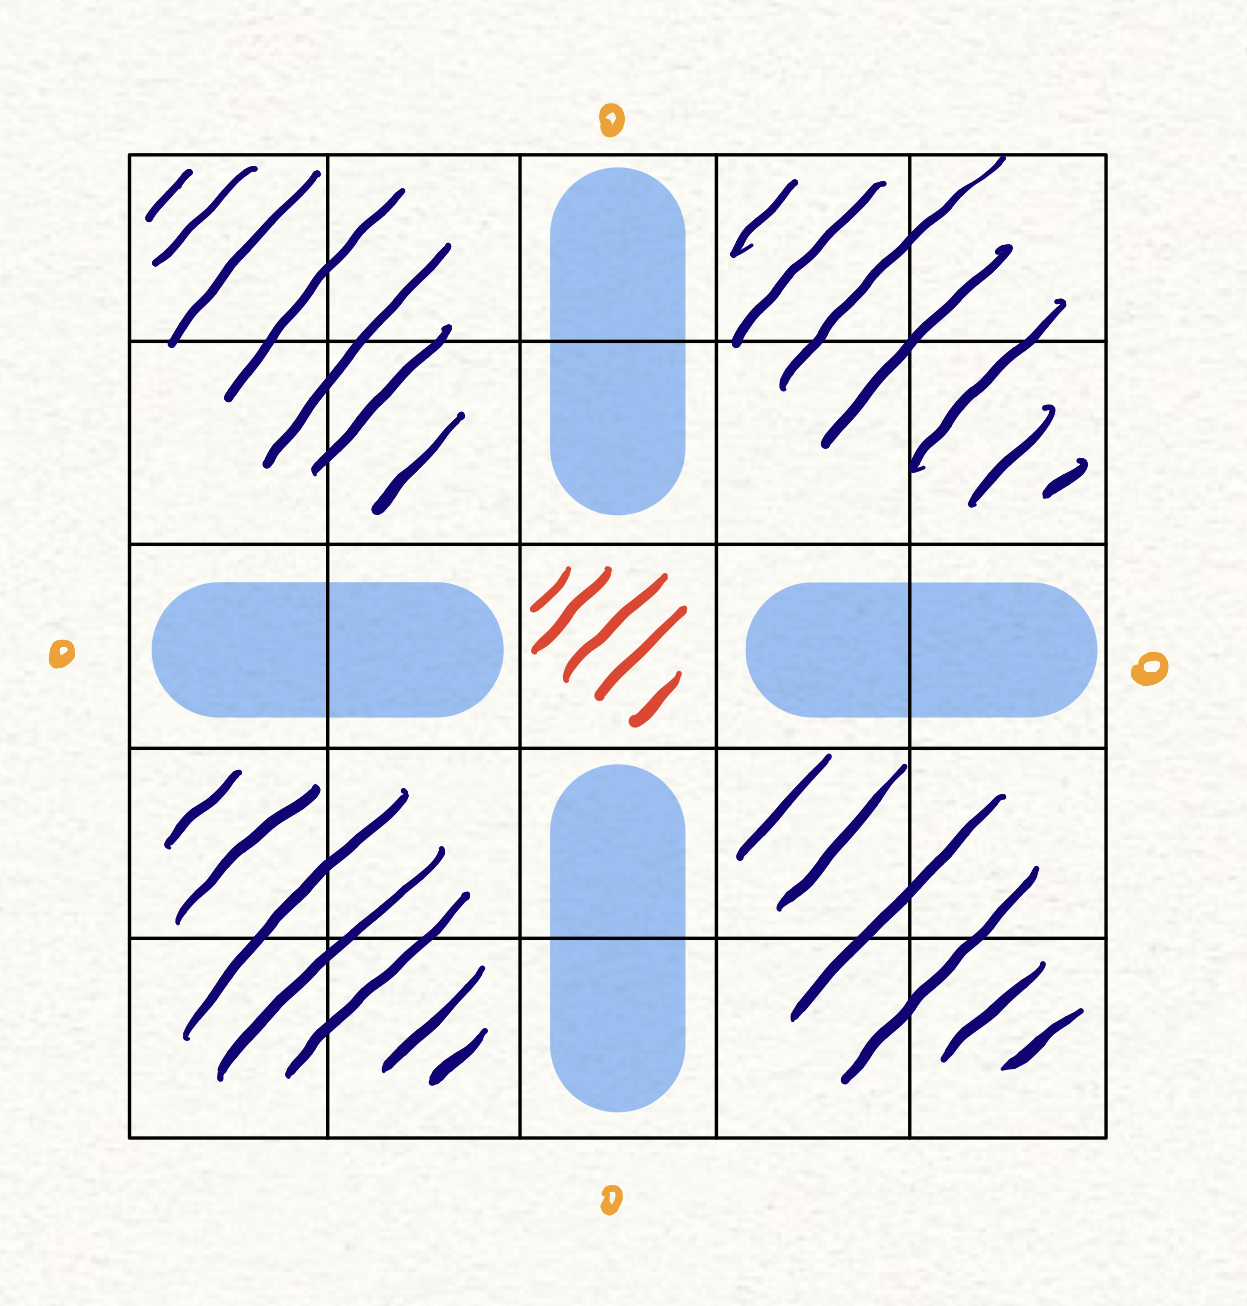
\includegraphics[width=0.5\textwidth]{./figs/h2_illustration.jpg}
            \caption{启发式函数$h_2$图示}
        \end{figure}
        每个区域只考虑从区域相邻的通道口进入,即位于角的四个区域考虑两个通道口,
        荧光笔所示的竖条区域只考虑一个通道口,正中心的不考虑通道。
        可以看到,采用$h_2$的算法速度很快。
    \end{enumerate}

    \section{CSP工作调度问题}
    \subsection{变量集合、值域集合、约束集合}
    以下集合为对应我具体实现的集合,对于不同的集合定义,可能有不同的实现。
    \paragraph{变量集合}
    对于$n$个工人的工作调度,一共有$7\times n$个变量,分别对应某一天某个工人。
    \paragraph{值域集合}
    对于每个变量,值域为$\{0, 1\}$,即在某一天某一个工人是否值班。
    \paragraph{约束集合}
    \begin{itemize}
        \item 每个工人每周必须休息2天或两天以上
        \item 每个工人每周不可以连续休息3天(不考虑跨周情况)
        \item 一周七天每天都要安排工人值班
        \item 每天安排至少$m(0 \leq m \leq n)$个人值班。
        \item 每天至少要有一名级别为senior的工人值班。
        \item 对于每个工人,不想与$k(0 \leq k < n)$名工人同一天工作,分别为$w_1, w_2, \cdots w_k$。
    \end{itemize}
    \subsection{算法主要思想}
    算法整体上采用回溯搜索,从分配表中按照某种顺序选择未赋值变量,
    遍历该变量在当前分配表及约束下的所有可能取值,并对当前状态进行推理(采用前向检验),
    在失败(即某一变量没有可能的取值)时失败,
    进行回溯。
    \subsection{局部搜索算法}
    局部搜索基本思想如以下伪代码所示:
    \begin{algorithm}[H]
        \caption{Local Search}
        \begin{algorithmic}
            \Require{$csp, max\_steps$}
            \State $assignment \gets \text{an initial complete assignment for csp}$
            \For{$i \gets 1$ to $max\_steps$}
                \If{assignment is consistent}
                    \State \Return $assignment$
                \EndIf
                \State $var \gets \text{a randomly chosen conflicted variable from } csp.\text{VARIABLES}$
                \State $value \gets \text{the value} v \text{for } var \text{that minimizes } \text{CONFLICTS}(var, v, assignment, csp)$
                \State \Comment{CONFLICTS can be defined as the sum of the number of violations of constraint}
                \State $\text{set } var = value \text{ in } assignment$
            \EndFor
            \State \Return $Failure$
        \end{algorithmic}
    \end{algorithm}


    \subsection{优化}
    主要的优化部分就是实现前向检验,对于某一个状态,判断所有未赋值变量是否有确定的值,
    例如当天有不想同一天工作的人工作,那就可以确定这一天这个工人所对应的变量为0(即不工作),等等。
    效果如下:
    \begin{figure}[H]
        \centering
        \subfigure{
            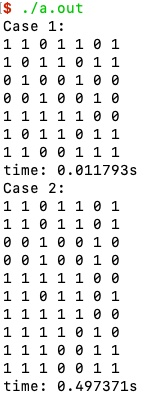
\includegraphics[height=10cm]{./figs/unoptimized.jpg}
        }
        \subfigure{
            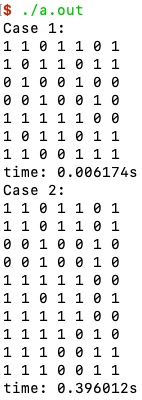
\includegraphics[height=10cm]{./figs/optimized.jpg}
        }
        \caption{未优化(左)与优化后(右)的对比}
    \end{figure}
    其中输出格式并非要求格式,输出文件中为要求格式。
    可以看到,还是有一定的优化效果,相信当问题规模更大时(搜索范围更大时),前向检验的效果会更加明显。
\end{document}
